%-%-%-%--%-%-%-%-%-%--%-%-%--%-%
% Author  : Tiago Chedraoui Silva
% License : GNU GPL v.3
% Title   : Mapa mental
% Tags    : mindmap, layers
%-%-%-%-%-%-%-%-%-%--%-%-%-%-%-%
\documentclass{article}
\usepackage{tikz,times}
\usepackage[paperwidth=55cm,paperheight=42cm,left=1cm,top=1cm]{geometry}
\usetikzlibrary{mindmap,backgrounds}

\pagestyle{empty}
\begin{document}
\centering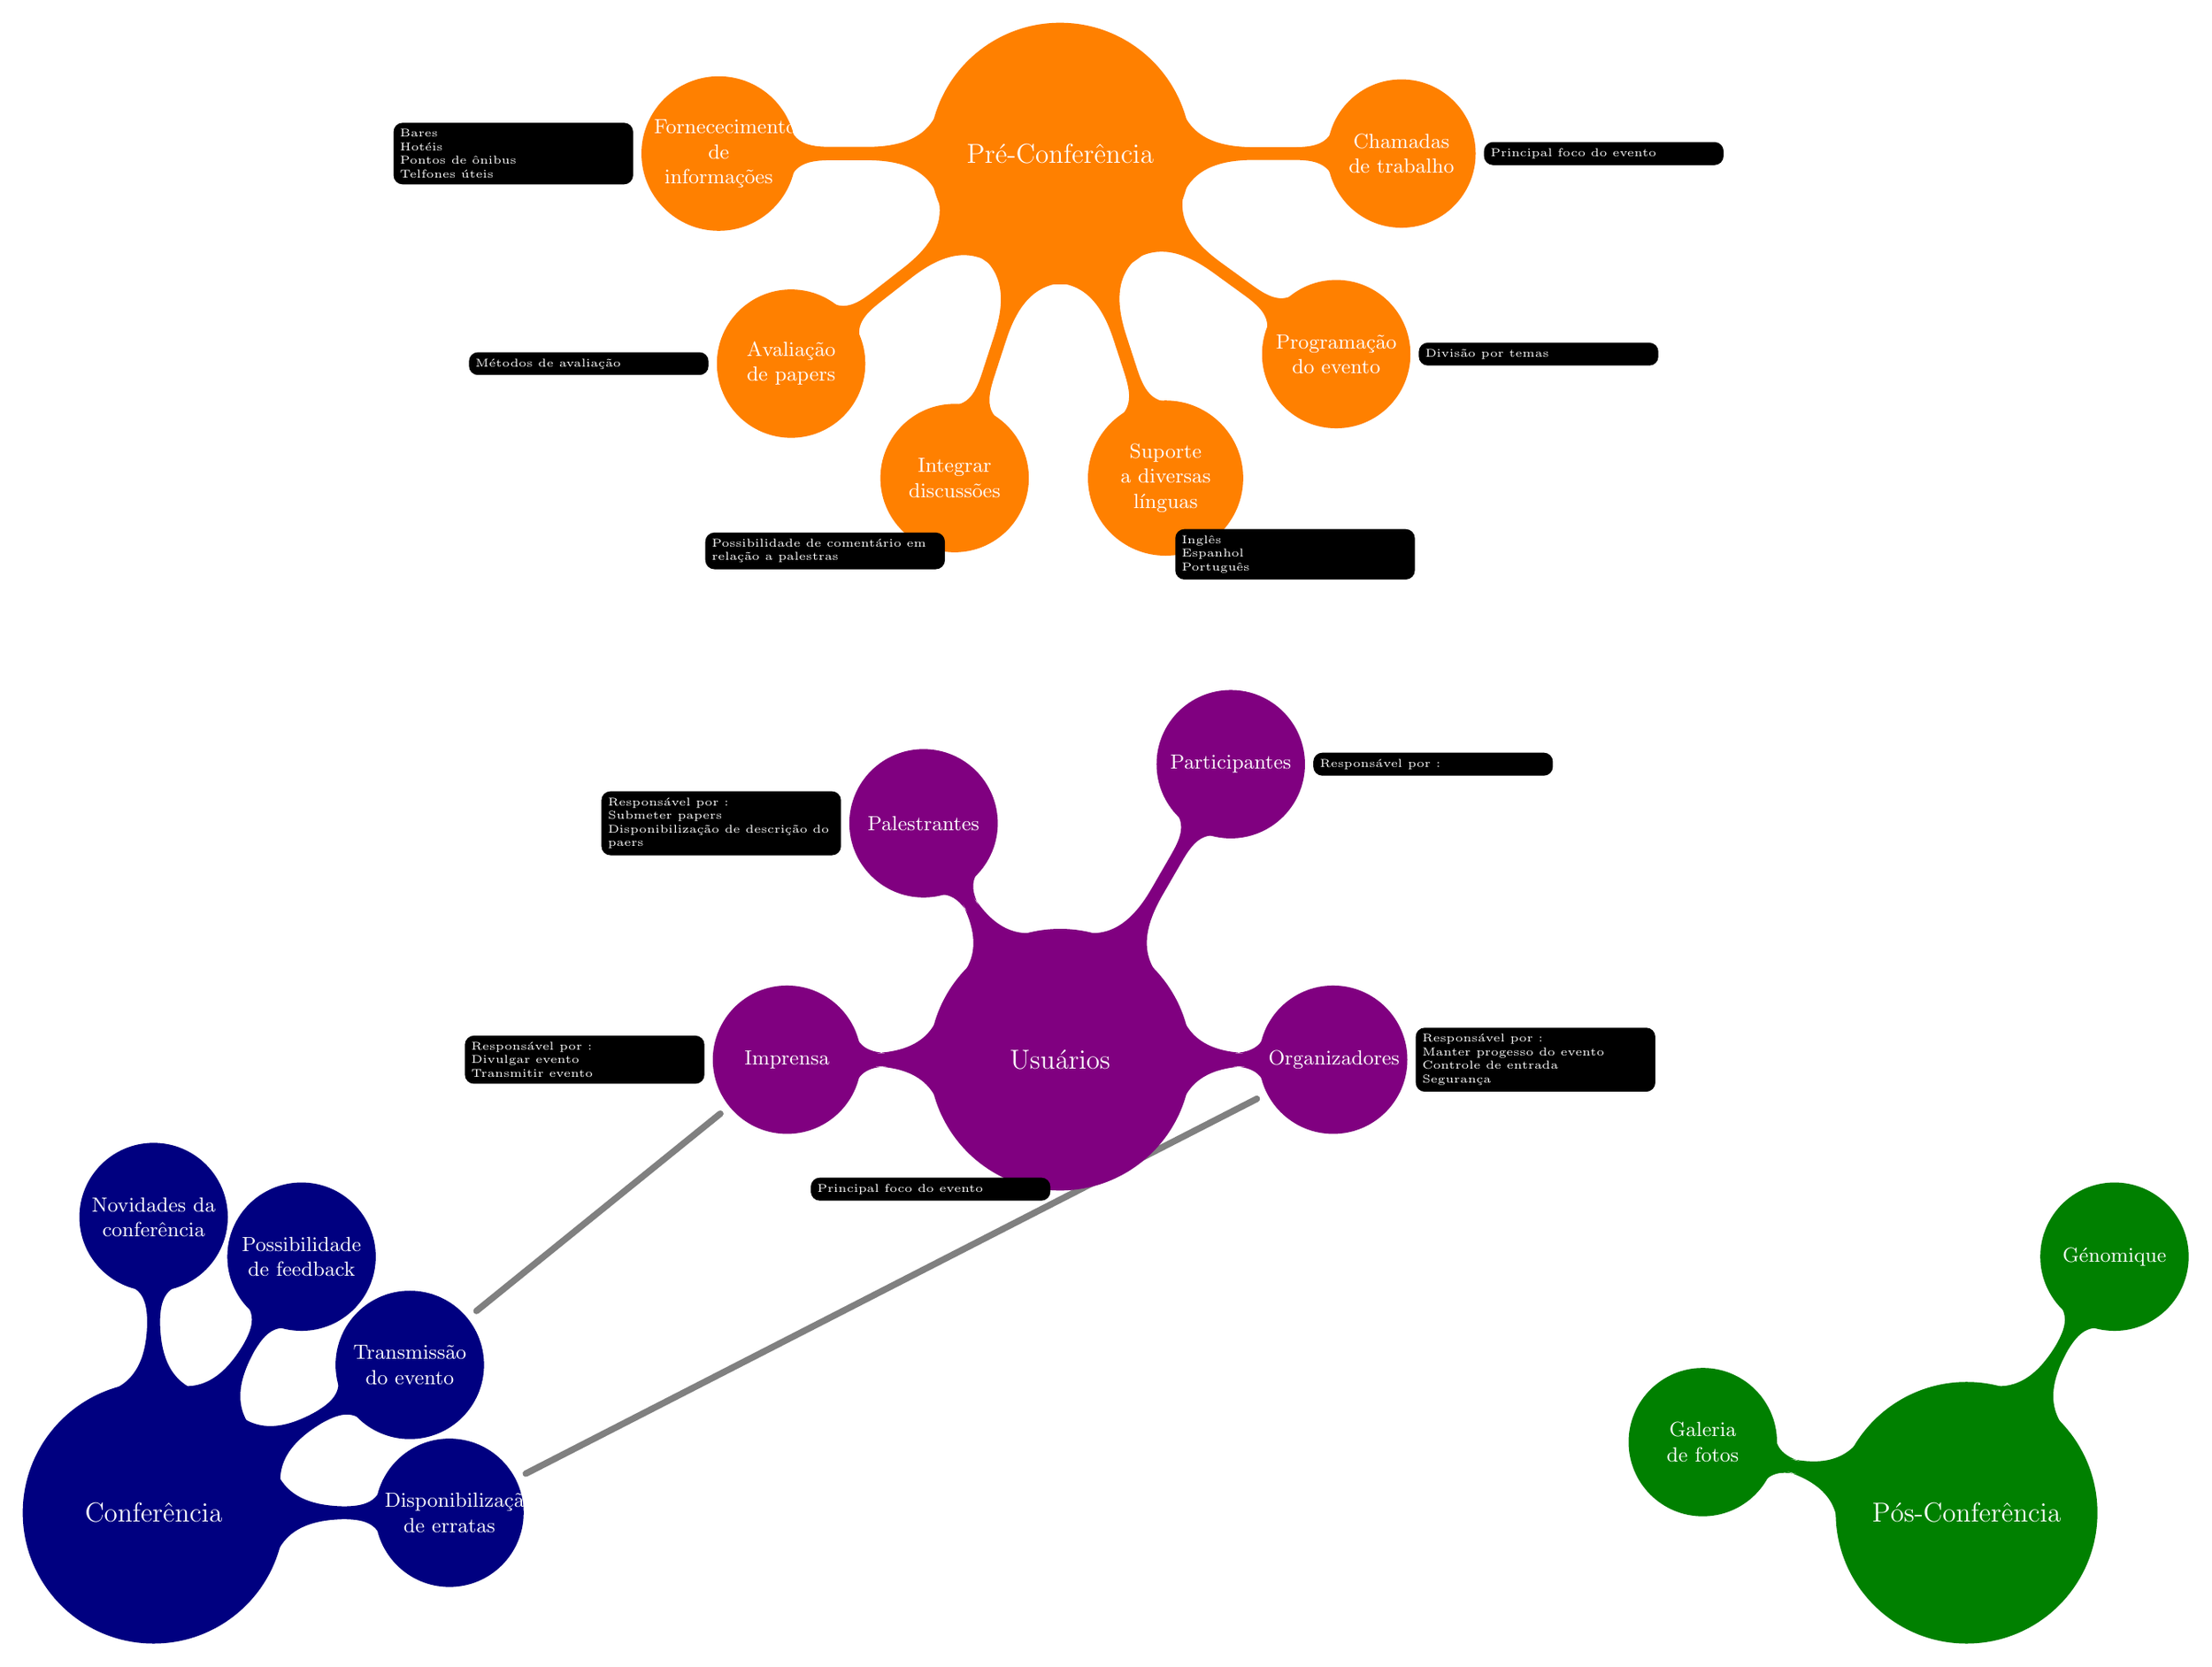
\begin{tikzpicture}[mindmap,
  level 1 concept/.append style={level distance=130,sibling angle=30},
  extra concept/.append style={color=blue!50,text=black},every annotation/.style={fill=black}]

  % Applied area:Pre-conferencia (one subfield)

  \begin{scope}[mindmap, concept color=orange, text=white,,every annotation/.style={fill=black}]
    \node [concept] {{Pr\'e-Confer\^encia}}%[clockwise from=-5] 
      child  [grow=0, level distance=150]{node [concept] (prc-trab) {Chamadas de trabalho}}
      child  [grow=-36, level distance=150]{node [concept] (prc-prog) {Programa\c{c}\~ao do evento}}
      child  [grow=-72, level distance=150]{node [concept] (prc-ling) {Suporte a diversas l\'inguas}}
      child  [grow=-108, level distance=150]{node [concept] (prc-forum) {Integrar discuss\~oes}}
      child  [grow=-142, level distance=150]{node [concept] (prc-aval) {Avalia\c{c}\~ao de papers}}
      child [grow=-180, level distance=150] {node [concept] (prc-info) {Fornececimento de informa\c{c}\~oes}};

      \node [annotation,right] at (prc-trab.east)
      {Principal foco do evento};
      \node [annotation,right] at (prc-ling.south)
      {Ingl\^es\\Espanhol\\Portugu\^es};
      \node [annotation,left] at (prc-forum.south)
      {Possibilidade de comentário em rela\c{c}\~ao a palestras};
   \node [annotation,right] at (prc-prog.east)
      {Divisão por temas};
   \node [annotation,left] at (prc-aval.west)
      {M\'etodos de avalia\c{c}\~ao};

   \node [annotation,left] at (prc-info.west)
      {Bares\\Hotéis\\Pontos de \^onibus\\Telfones \'uteis};


  \end{scope}


  % Applied area:Pos conferencia  (one subfield)

  \begin{scope}[mindmap, concept color=green!50!black,text=white]
    \node [concept] at (14.0,-21) {P\'os-Confer\^encia} 
      child [grow=165, level distance=120] 
        {node [concept] (med) {Galeria de fotos}}
      child [grow=60] 
        {node [concept] (gen) {G{\'e}nomique}};
  \end{scope}

  % Applied area:usuários  (one subfield)

  \begin{scope}[mindmap, concept color=violet, text=white,every annotation/.style={fill=black}]
    \node [concept](usr) at (0,-14.0)  {Usu{\'a}rios}
      child [grow=0, level distance=120] 
        {node [concept] (org) {Organizadores}}
    child [grow=60, level distance=150] 
        {node [concept] (upar) {Participantes}}
      child [grow=120, level distance=120] 
        {node [concept] (upal) {Palestrantes}}
      child [grow=180, level distance=120] 
        {node [concept] (uimp) {Imprensa}};
      \node [annotation,left] at (usr.south)
      {Principal foco do evento};
    \node [annotation,left] at (uimp.west)
      {Respons\'avel por :\\Divulgar evento\\ Transmitir evento};
    \node [annotation,right] at (upar.east)
      {Respons\'avel por :\\};
    \node [annotation,left] at (upal.west)
      {Respons\'avel por :\\Submeter papers\\Disponibilização de descrição do paers  };
  \node [annotation,right] at (org.east)
      {Respons\'avel por :\\Manter progesso do evento\\Controle de entrada\\Segurança };

   
\end{scope}


%conferencia
  \begin{scope}[mindmap, concept color=blue!50!black, text= white]

    \node [concept, text=white] at(-14,-21)% (5.2,-10.8) 
      {Confer\^encia} 
      [clockwise from=150]
      child [grow=90] {node [concept] (c-nov) {Novidades da confer\^encia}}
      child [grow=60 level distance=125] 
        {node [concept] (c-feed) {Possibilidade de feedback}}
      child [grow=0] 
        {node [concept] (c-err) {Disponibiliza\c{c}\~ao de erratas}}
      child [grow=30] {node [concept](c-tr) {Transmiss\~ao do evento}};
  \end{scope}

  % Connections of researchers to applied subfields

  \begin{pgfonlayer}{background}
   % \draw [circle connection bar]
   \draw [concept connection ]
     (c-tr) edge (uimp)
     (c-err) edge (org);
  
 \end{pgfonlayer}
\end{tikzpicture}

\end{document}
